\documentclass[11pt, a4paper]{article}
\newcommand{\HomeworkHeader}{L02\_04-L02\_06}
% Shared LaTeX preamble for homework/*/main.tex

% --- Base layout ---
\usepackage[a4paper, top=2.5cm, bottom=2.5cm, left=2cm, right=2cm]{geometry}
\usepackage{fontspec}
\usepackage{xeCJK} % CJK fallback to avoid missing glyphs in Latin fonts
\usepackage{amsmath, amssymb, amsthm}
\usepackage{mathtools}
\usepackage{fancyhdr}
\usepackage{lastpage}
\usepackage[svgnames]{xcolor}
\usepackage{tikz}
\usetikzlibrary{automata, positioning, arrows.meta, bending, backgrounds}
\usepackage{pgfplots}
\pgfplotsset{compat=1.18}
\usepackage[most]{tcolorbox}
\usepackage{enumitem}

% --- Languages & fonts ---
\usepackage[english]{babel}
\babelprovide[import, main]{chinese}

\babelfont{rm}[UprightFont=*, BoldFont=* Bold, ItalicFont=* Italic, Scale=1.05]{Linux Libertine O}
\babelfont{sf}[UprightFont=*, BoldFont=* Bold, Scale=1.05]{Linux Biolinum O}
\babelfont[chinese]{rm}[
    UprightFont=*-Regular,
    BoldFont=*-Bold,
    ItalicFont=*-Regular,
    BoldItalicFont=*-Bold
]{Noto Serif CJK SC}
\babelfont[chinese]{sf}[
    UprightFont=*-Regular,
    BoldFont=*-Bold
]{Noto Sans CJK SC}
\babelfont{tt}{Noto Sans Mono}
\babelfont[chinese]{tt}{Noto Sans Mono CJK SC}

% xeCJK font setup (kept consistent with babelfont)
\setCJKmainfont{Noto Serif CJK SC}
\setCJKsansfont{Noto Sans CJK SC}
\setCJKmonofont{Noto Sans Mono CJK SC}

% --- Colors ---
\definecolor{primaryColor}{RGB}{46, 52, 64}
\definecolor{accentColor}{RGB}{94, 129, 172}
\definecolor{boxFill}{RGB}{236, 240, 241}
\definecolor{solLine}{RGB}{163, 190, 140}
\definecolor{expandColor}{RGB}{191, 97, 106}

% --- TikZ styles (DFA / NFA / PDA) ---
\tikzset{
    dfa_state/.style={
        state,
        thick,
        draw=accentColor,
        fill=boxFill,
        text=primaryColor,
        minimum size=1.1cm
    },
    dfa_edge/.style={
        ->,
        >=stealth,
        thick,
        draw=primaryColor,
        auto
    },
    pda_node/.style={
        state,
        thick,
        draw=accentColor,
        fill=boxFill,
        text=primaryColor,
        minimum size=1.2cm
    },
    pda_edge/.style={
        ->,
        >=stealth,
        thick,
        draw=primaryColor,
        auto
    },
    rule_expand/.style={
        pda_edge,
        draw=expandColor,
        text=expandColor
    },
    rule_match/.style={
        pda_edge,
        draw=solLine,
        text=solLine!80!black
    }
}

% --- Header / footer ---
\pagestyle{fancy}
\fancyhf{}
\lhead{\color{accentColor}\textbf{形式语言与自动机作业}}
\rhead{\color{primaryColor}\textbf{\HomeworkHeader}}
\cfoot{\small 第 \thepage \ 页,共 \pageref{LastPage} 页}
\setlength{\headheight}{24pt}
\addtolength{\topmargin}{-12pt}
\setlength{\emergencystretch}{2em}
\renewcommand{\headrulewidth}{0.4pt}
\renewcommand{\headrule}{\hbox to\headwidth{\color{accentColor}\leaders\hrule height \headrulewidth\hfill}}

% --- Problem box ---
\newtcolorbox[auto counter]{problem}[1][]{
    enhanced,
    breakable,
    colback=boxFill,
    colframe=accentColor,
    coltitle=white,
    fonttitle=\bfseries\large,
    title={题目 ~\thetcbcounter \quad #1},
    boxrule=0.5mm,
    arc=3mm,
    drop shadow=black!15!white,
    attach boxed title to top left={xshift=0.5cm, yshift*=-3mm},
    boxed title style={colback=accentColor}
}

% --- Solution environment ---
\newenvironment{solution}{
    \par\vspace{10pt}
    \noindent\textbf{\color{solLine} \Large \textit{Solution.}} \par
    \begingroup\color{primaryColor}\sloppy
    \leftskip1em \rightskip1em
    \noindent\rule{\textwidth}{0.4pt}
    \par\vspace{5pt}
}{
    \par\vspace{10pt}
    \noindent\rule[0.5ex]{\textwidth}{0.1pt}
    \endgroup
    \vspace{1.2cm}
}

% --- Title ---
\newcommand{\makeCustomTitle}[1]{
    \begin{center}
        \vspace*{1cm}
        {\Huge \bfseries \color{primaryColor} 作业 #1}\\
        \vspace{0.5cm}
        {\Large \color{accentColor} \today}
        \vspace{1.2cm}
    \end{center}
}


\begin{document}

\makeCustomTitle{L2.4 - L2.6:CFG 与二义性}

% --- Problem 1 ---
\begin{problem}
分别构造产生下列语言的 CFG:
\begin{enumerate}[label=(\arabic*)]
    \item $\{1^n0^m \mid n \ge m \ge 1\}$
    \item $\{1^n0^{2m}1^n \mid n,m \ge 1\}$
    \item $\{1^n0^n1^m0^m \mid n,m \ge 1\}$
    \item 含有相同个数的 $0$ 和 $1$ 的所有 $01$ 串
    \item 字母表 $\{1,2,3\}$ 上的所有正则表达式
\end{enumerate}
\end{problem}

\begin{solution}
\textbf{(1) $\{1^n0^m \mid n \ge m \ge 1\}$}

思路:先生成至少一个匹配对 $10$,再在左侧额外补若干个 $1$。
\[
S \to 1S \mid T,\qquad
T \to 10 \mid 1T0.
\]
其中 $T$ 生成 $1^m0^m\ (m\ge 1)$,$S$ 在其左侧再补若干个 $1$,得到 $1^{m+k}0^m$。

\textbf{(2) $\{1^n0^{2m}1^n \mid n,m \ge 1\}$}

思路:外层保证两侧 $1$ 的个数相等且至少 1,对中间部分生成偶数个 $0$ 且至少 2。
\[
S \to 1A1,\qquad
A \to 1A1 \mid B,\qquad
B \to 00 \mid 00B.
\]
$B$ 生成 $0^{2m}(m\ge 1)$,$A$ 可继续对称包裹额外的 $1$。

\textbf{(3) $\{1^n0^n1^m0^m \mid n,m \ge 1\}$}

两个独立的“相等计数”串连接:
\[
S \to UV,\qquad
U \to 10 \mid 1U0,\qquad
V \to 10 \mid 1V0.
\]
其中 $U$ 生成 $1^n0^n(n\ge 1)$,$V$ 生成 $1^m0^m(m\ge 1)$。

\textbf{(4) 相同个数的 $0$ 与 $1$ 的所有 $01$ 串}

经典文法(允许任意穿插):
\[
S \to SS \mid 0S1 \mid 1S0 \mid \epsilon.
\]
该文法生成所有 $0$ 与 $1$ 数目相等的二进制串。

\textbf{(5) $\{1,2,3\}$ 上的所有正则表达式}

把正则表达式按“并、连接、星号、括号、字面符号、空串”归纳生成:
\[
\begin{aligned}
R &\to R + C \mid C,\\
C &\to CF \mid F,\\
F &\to A^* \mid A,\\
A &\to (R) \mid 1 \mid 2 \mid 3 \mid \epsilon.
\end{aligned}
\]
(若课程中不允许显式 $\epsilon$ 作为基本符号,可去掉 $A\to\epsilon$,改用其它约定。)
\end{solution}

% --- Problem 2 ---
\begin{problem}
对例 2 中的文法 $G$,给出字符串 $w=\texttt{abbb aab bab a}$(即 $\texttt{abbb aabbbaba}$)的派生树,并利用该派生树找出该字符串的最左派生。
\end{problem}

\begin{solution}
课件“例 2”的文法为:
\[
S\to abB,\qquad A\to aaBb\mid \epsilon,\qquad B\to bbAa.
\]
题面字符串按连续写法为 $w=\texttt{abbbaabbaba}$。

\textbf{一条成功派生(同时也是最左派生)}:
\[
\begin{aligned}
S
&\Rightarrow abB\\
&\Rightarrow ab\,bbAa\\
&\Rightarrow ab\,bb\,aaBb\,a\\
&\Rightarrow ab\,bb\,aa\,bbAa\,b\,a\\
&\Rightarrow \texttt{abbbaabbaba}\qquad(\text{用 }A\Rightarrow \epsilon).
\end{aligned}
\]

\textbf{派生树(用产生式展开顺序画出)}:

\begin{center}
\begin{tikzpicture}[
  level distance=14mm,
  sibling distance=10mm,
  every node/.style={font=\small},
  edge from parent/.style={draw=primaryColor, thick}
]
\node {$S$}
  child { node {$a$} }
  child { node {$b$} }
  child { node {$B$}
    child { node {$b$} }
    child { node {$b$} }
    child { node {$A$}
      child { node {$a$} }
      child { node {$a$} }
      child { node {$B$}
        child { node {$b$} }
        child { node {$b$} }
        child { node {$A$} }
        child { node {$a$} }
      }
      child { node {$b$} }
    }
    child { node {$a$} }
  };
\end{tikzpicture}
\end{center}
\end{solution}

\section*{二义性与派生关系总结}

% --- Problem 3 ---
\begin{problem}
请总结:
\begin{enumerate}[label=(\arabic*)]
    \item 非二义性 CFG 的句型派生、最左/最右派生以及派生树之间的关系
    \item 二义性文法中派生、最左/最右派生以及派生树之间的关系
    \item 语言的固有二义性与文法的二义性之间的关系
\end{enumerate}
\end{problem}

\begin{solution}
\textbf{(1) 非二义性 CFG}
\begin{itemize}
    \item 对于同一个串 $w$,\textbf{派生树唯一}(忽略同构的画法差异)。
    \item 由派生树可以唯一确定它的最左派生与最右派生(每一步展开当前最左/最右的非终结符)。
    \item 因为派生树唯一,所以最左派生、最右派生在“产生式选择序列”意义下也是唯一的(具体中间句型的书写可能等价重排,但结构不变)。
\end{itemize}

\textbf{(2) 二义性文法}
\begin{itemize}
    \item 存在某个串 $w$ 具有\textbf{至少两棵不同的派生树}。
    \item 不同派生树对应不同的最左派生/最右派生;反之,若存在两条不同的最左派生(或最右派生)导出同一终结串,则必然二义。
    \item 二义性体现在“结构”上:虽然都能导出同一串,但解析结构不同(例如不同的运算优先级/结合性)。
\end{itemize}

\textbf{(3) 固有二义性 vs 文法二义性}
\begin{itemize}
    \item \textbf{文法二义性}:某个特定 CFG 是二义的(存在串有多棵派生树)。
    \item \textbf{语言固有二义性}:某个语言 $L$ 的\textbf{所有} CFG 都是二义的;也就是说不存在能生成 $L$ 的非二义 CFG。
    \item 因此:文法二义 $\not\Rightarrow$ 语言固有二义(可能换个文法就不二义);但语言固有二义 $\Rightarrow$ 任意生成它的文法都二义。
\end{itemize}
\end{solution}

% --- Problem 4 ---
\begin{problem}
对例 7 给定的文法,采用穷举搜索法对字符串 $\texttt{aab dabb}$(即 $\texttt{aabdabb}$)进行解析。
\end{problem}

\begin{solution}
课件“例 7”中的文法(与课件给出的派生树相符)为:
\[
S\to aAb \mid bBa,\qquad
A\to aAb \mid bBa,\qquad
B\to d.
\]
目标串为 $w=\texttt{aabdabb}$(即 $a\,a\,b\,d\,a\,b\,b$)。

\textbf{穷举搜索法(按“每层展开当前最左变量”的思路)}

从根开始:
\[
S \Rightarrow aAb
\]
为了匹配以 $aa$ 开头,继续展开最左变量 $A$ 取 $A\Rightarrow aAb$:
\[
aAb \Rightarrow aaAbb.
\]
此时需要在中间产生 $d$,选择 $A\Rightarrow bBa$:
\[
aaAbb \Rightarrow aabBabb.
\]
最后用 $B\Rightarrow d$:
\[
aabBabb \Rightarrow aabdabb,
\]
匹配成功。

\textbf{对应派生树}:
\begin{center}
\begin{tikzpicture}[
  level distance=14mm,
  sibling distance=12mm,
  every node/.style={font=\small},
  edge from parent/.style={draw=primaryColor, thick}
]
\node {$S$}
  child { node {$a$} }
  child { node {$A$}
    child { node {$a$} }
    child { node {$A$}
      child { node {$b$} }
      child { node {$B$}
        child { node {$d$} }
      }
      child { node {$a$} }
    }
    child { node {$b$} }
  }
  child { node {$b$} };
\end{tikzpicture}
\end{center}

\textbf{最左派生序列}(与上面的搜索路径一致):
\[
S\Rightarrow aAb\Rightarrow aaAbb\Rightarrow aabBabb\Rightarrow aabdabb.
\]
\end{solution}

\end{document}
